%%%%%%%%%%%%%%%%%%%%%%%%%%%%%%%%%
%
%       EXERCÍCIO
%
%%%%%%%%%%%%%%%%%%%%%%%%%%%%%%%%%

\ifdefstring{\atividade}{prova}{%
    \ifdefstring{\modo}{objetivo}{%
        \renewcommand{\valorquestao}{\ValorQObj\ ponto}
    }{%
        \renewcommand{\valorquestao}{\ValorQDisc\ pontos}
    }%
}%

\begin{exercicioBanco}[\valorquestao]
Considere a reta numérica.
%
\vspace{15pt}
\begin{center}
    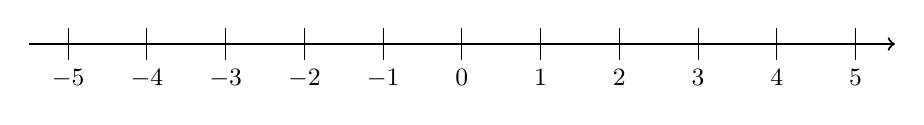
\begin{tikzpicture}[scale=1]

    % Linha principal com seta
    \draw[->, thick] (-5.5,0) -- (5.5,0);

    % Marcas e números
    \foreach \x in {-5,-4,-3,-2,-1,0,1,2,3,4,5}
    {
        \draw (\x,0.2) -- (\x,-0.2);
        \node[below] at (\x,-0.2) {\small $\x$};
    }
    \end{tikzpicture}
\end{center}
%
O número \(-\dfrac{17}{5}\) foi marcado entre que pontos dessa reta numérica?

% Define as alternativas
\newcommand{\alternativas}{%
    \begin{center}
        \begin{tabularx}{\textwidth}{XXXXX}
            (a) \(2\) e \(3\). &
            (b) \(3\) e \(4\). &
            (c) \(-3\) e \(-2\). &
            (d) \(-4\) e \(-3\). &
            (e) \(-5\) e \(-4\).
        \end{tabularx}
    \end{center}
}

% Define a resposta correta
\newcommand{\resposta}{D}

% Lógica condicional para exibição
\ifdefstring{\atividade}{lista}{%
    \alternativas
    \vspace{0.5em}
    
    \noindent\textbf{Resposta:} letra \textbf{\resposta}.
}{%
    \ifdefstring{\modo}{objetivo}{%
        \alternativas
    }{%
        % modo = discursiva → não mostra alternativas
    }
}
\end{exercicioBanco}

